
\documentclass[12pt]{amsart}   % LaTeX with AMS style; 12 point for old eyes

\usepackage{amsmath,amssymb,amsfonts}   % For better support of math
\usepackage{graphicx}	        % Enable for eps and pdf figures, if they occur
\usepackage{caption}
\usepackage{float}
\usepackage{subcaption}
\usepackage{hyperref} % Enable embedded hyperlinks.
\hypersetup{
	hidelinks, colorlinks, linkcolor=black, citecolor=black, urlcolor=red
}
        
% Commands to force sequential numbering:

\newtheorem{theorem}{Theorem}[section]
\newtheorem{proposition}[theorem]{Proposition}
\newtheorem{lemma}[theorem]{Lemma}
\newtheorem{definition}[theorem]{Definition}
\newtheorem{examples}[theorem]{Examples}
\newtheorem{remarks}[theorem]{Remarks}
\newtheorem{corollary}[theorem]{Corollary}
\newtheorem{remark}[theorem]{Remark}
\newtheorem{example}[theorem]{Example}
\newtheorem{conjecture}[theorem]{Conjecture}

% Define abs norm, paren, bracket, cbracket, and innerproduct
\usepackage{mathtools}
\DeclarePairedDelimiter\tempabs{\lvert}{\rvert}
\DeclarePairedDelimiter\tempnorm{\lVert}{\rVert}
\DeclarePairedDelimiter\tempinnerproduct{\langle}{\rangle}
\DeclarePairedDelimiter\tempparen{(}{)}
\DeclarePairedDelimiter\tempbracket{[}{]}
\DeclarePairedDelimiter\tempcbracket{\{}{\}}
\DeclareMathOperator*{\argmin}{arg\,min}
\DeclareMathOperator*{\argmax}{arg\,max}
% Swap * functionality
\makeatletter
\def\abs{\@ifstar{\tempabs}{\tempabs*}}
\def\norm{\@ifstar{\tempnorm}{\tempnorm*}}
\def\innerproduct{\@ifstar{\tempinnerproduct}{\tempinnerproduct*}}
\def\paren{\@ifstar{\tempparen}{\tempparen*}}
\def\bracket{\@ifstar{\tempbracket}{\tempbracket*}}
\def\cbracket{\@ifstar{\tempcbracket}{\tempcbracket*}}
\makeatother

% blackboard bold , for ``complex,'' etc
\newcommand{\C}{\mathbb C} 
\newcommand{\R}{\mathbb R} 
\newcommand{\Z}{\mathbb Z}
\newcommand{\Q}{\mathbb Q}
\newcommand{\N}{\mathbb N}

% Add fig with caption command. Inputs: {path}{caption}{label}
\newcommand{\includefig}[3]{
  \begin{figure}[H]
    \begin{center}
      \includegraphics[width=4in,height=3in,keepaspectratio]{#1}
    \end{center}
  \vspace{-.2in} % corrects bad spacing
  \caption{#2.\label{fig:#3}}
  \end{figure}
}

\newcommand{\bvec}[1]{\mathbf{#1}}
\newcommand{\bhat}[1]{\mathbf{\hat{#1}}}

\begin{document}

\graphicspath{ {figures/} }

\title[Optimal Paths in R2]{Optimal Particle Paths Around Points in $\R^2$ with Constrained Acceleration} 
 
\author{Jonathan Allen, John Wang}
\date{\today}

\maketitle

\subsection*{Abstract}

Optimal particle paths in $\R^2$ between points and around points are investigated in this paper. A paramerization of a particle's motion around a point is defined. From this parameterization, we derive a general solution for an optimal path with constant speed between 2 points. The results of this paper can by applied towards calculating optimal object trajectories in physics when acceleration is constrained. 

\section{Introduction}
The problem of finding fastest paths between two points (let's call them A and B) is interesting because many attributes of a fastest path are intuitively obvious, but rigorously proving them is much more difficult. One's first assumption would be that the fastest path between A and B, would be to travel in a straight line from A to B. This would be true in the simple case where the turning rate is not constrained, but it is not true in the general case when a particle has a constrained turning rate and starts with some nonzero velocity not directed towards B. In the general case, it is easier to turn towards B, the further one is away from it, so there is the possibility that it would be fastest for the particle to turn away from B for a short period of time, so that it can then turn towards it more quickly. In fact, if the particle is too close to B, it won't have time to turn towards it, and will pass by B. 

\subsection{The Problem (more precise terms will be defined later)}

Given a particle in $\R^2$ starts at a position A in with an initial velocity, what is the path in for the particle to take to reach a final position B, such that the time spent traveling from A to B is minimized. The particle can have restrictions on its position, velocity, and acceleration. Our model problem has fixed speed and a bounded turning rate.

\subsection{Motivation}

The problem of finding a fastest path for a particle with constant speed is useful because it is identical to the problem of finding a shortest path given constraints on the radius of curvature of the path, which appears in fields such as physics and computational geometry. 

Intuitively, one could imagine a race car driver navigating a racetrack with constant speed, as a physical example of the problem. In fact, this example directly motivates our problem, because a race car driver has a limited turning rate which is created by friction between the wheels and the ground.

Understanding how to find fastest paths for a particle with constant speed will also provide insight into solving even more complicated problems which may have varying speed and more dimensions such as spacecraft trajectories.

\subsection{Outline}

We first present a modified polar coordinate system to represent the particle's motion around a point and then derive a set of differential equations governing the motion of the particle in this coordinate system. This allows us to devise some simple lemmas about the motion of the particle, and draw some conclusions about fastest paths.

\section{Notation}
\subsection{Vectors}

\begin{description}
  \item[$a$] Scalar quantity.
  \item[$\bvec{a}$] Vector in n-dimensional space. $\norm{\bvec{a}} = a$.
  \item[$\bhat{a}$] Unit vector in n-dimensional space. $\bhat{a} = \bvec{a}/a$ and $\norm{\bhat{a}} = 1$.
\end{description}

\subsection{Angles}

Since many of the theorems in this paper involve polar coordinates, we define two different types of angle measurements: a standard measurement, and a directional measurement (all angles are measured in radians).

In the standard measurement, angles are in $[0, 2\pi]$ and are measured counterclockwise. In the directional measurement, angles are in $[-\pi, \pi]$ and the measurement direction is indicated by an arrow on the measurement.

\begin{figure}[H]
  \centering
  \begin{subfigure}[b]{0.4\textwidth}
    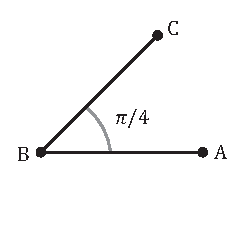
\includegraphics[width=\textwidth]{angle_def_1.eps}
    \caption{}
    \label{fig:angle-def-1}
  \end{subfigure}
  \qquad \qquad
  \begin{subfigure}[b]{0.4\textwidth}
    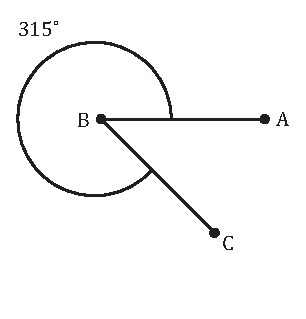
\includegraphics[width=\textwidth]{angle_def_2.eps}
    \caption{}
    \label{fig:angle-def-2}
  \end{subfigure}
  \caption{Standard angle notation (no arrow)}
\end{figure}

\begin{figure}[H]
  \begin{subfigure}[b]{0.4\textwidth}
    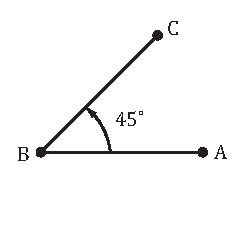
\includegraphics[width=\textwidth]{angle_def_3.eps}
    \caption{}
    \label{fig:angle-def-3}
  \end{subfigure}
  \qquad \qquad
  \begin{subfigure}[b]{0.4\textwidth}
    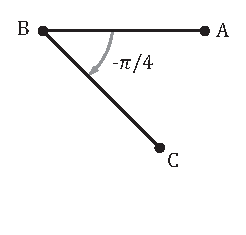
\includegraphics[width=\textwidth]{angle_def_4.eps}
    \caption{}
    \label{fig:angle-def-4}
  \end{subfigure}
  \caption{Directional angle notation (arrow)}
\end{figure}

\section{Particles and Paths}
In this section, we will provide some basic definitions about particles and paths. These will lay the groundwork for thinking about optimal paths. We will begin by defining the description of a particle and then define various types of paths along which a particle can travel.

\begin{definition}
A n-dimensional path $\gamma(t): \mathrm{R} \to \mathrm{R}^n$ is a function which maps a time $t \in \R$, $t \in [0, T_{f, \gamma}]$, to a position $\bvec{X} \in \mathrm{R}^n$. 
\end{definition}

\begin{definition}
  A n-dimensional particle, $p$, is an object with zero volume that travels along a n-dimensional path. The particle may have conditions on its position, velocity, and acceleration in $\R^n$.
\end{definition}

\begin{definition}
  A valid path $\gamma(t)$ for a particle $p$ is a path such that all conditions on the particle are satisfied at every point along the path.
\end{definition}

\begin{definition}
  A path between two points, $\bvec{X_1}$ and $\bvec{X_2}$ is a path, $\gamma(t)$ where $\gamma(0) = \bvec{X_1}$ and $\gamma(T_{f, \gamma}) = \bvec{X_2}$.
\end{definition}

\begin{definition}
  For a given particle, $p$, a fastest path, $\hat{\gamma}(t)$, between two points, $\bvec{X_1}$ and $\bvec{X_2}$, is a valid path such that $T_{f,\hat{\gamma}} \leq T_{f,\gamma}$ for all valid paths, $\gamma(t)$, between $\bvec{X_1}$ and $\bvec{X_2}$.
\end{definition}

\begin{definition}
  A particle's velocity is defined as 

  \[\bvec{v} \coloneqq \frac{d\bvec{X}}{dt}\]

  A particle's speed is $v$, and its direction of motion is $\bhat{v}$

\end{definition}

\begin{definition}
  A particle's acceleration is defined as 
  
  \[\bvec{a} \coloneqq \frac{d\bvec{v}}{dt}\]
\end{definition}

\begin{definition}
  The centripetal acceleration, $\bvec{a_c}$, of a particle, $p$, is the component of the acceleration of $p$ perpendicular to its direction of motion.

  In rectangular coordinates, the sign of $a_c$ is the projection of $\bhat{a_c}$ onto $\bhat{x}$. 

  In polar coordinates, the sign of $a_c$ is difined as the sign of the projection of $\bhat{a_c}$ onto $\bhat{r}$.
\end{definition}

\begin{definition}
  The tangential acceleration, $\bvec{a_t}$, of a particle, $p$, is the component of the acceleration of $p$ in its direction of motion, $\bhat{v}$. $a_t = \frac{ds}{dt}$.
\end{definition}

% -----------------------------------------------------------------------------

\subsection{Particle Motion in Polar Coordinates}

The motion of the 2-dimensional particles in this paper will be described in the polar coordinate system, shown in Figure \ref{fig:polar-param}.

\includefig{polar_param.eps}{A particle moving in 2-dimensional polar coordinate system centered at B}{polar-param}

\begin{lemma}
The time derivative of $\theta$ is given by
\[
\frac{d\beta}{dt} = \frac{a_c}{s}
\]
\end{lemma}

\begin{proof}

If we look at a point, $p$, subject to only centripetal acceleration, $a_c$, the change in $\bvec{v}$ over an infinitesimal time, $dt$, is shown in Figure \ref{fig:theta-deriv} (the two vectors, $\bvec{v}$ and $\bvec{v}+\bvec{dv}$, are superimposed). 

\includefig{theta_deriv.eps}{Tangential acceleration}{theta-deriv}

From the definition of $a_c$

\[
\frac{dv}{dt} = a_c
\]

So...
\[
\frac{d\beta}{dt} = \frac{a_c}{v}
\]
\end{proof}

The proof of the lemma in the case where $a_t$ is also nonzero is very similar, since the component of $\bvec{dv}$ in the direction $\bhat{v}$ is negligeable compared to $v$.

Returning again to Figure \ref{fig:polar-param}, the following equations can be derived

\begin{align}
  \frac{dr(t)}{dt}& = -s(t) \, \cos\paren{\theta(t)}\label{eq:r-deriv}\\
  \frac{d\phi(t)}{dt}& = s(t) \, \sin\paren{\theta(t)}\label{eq:phi-deriv}\\
  \frac{d\theta(t)}{dt}& = \frac{d\phi(t)}{dt} - \frac{a_c(t)}{s(t)}\\
  &= s(t) \, \sin\paren{\theta(t)} - \frac{a_c(t)}{s(t)}\label{eq:theta-deriv}\\
  \intertext{Applying the chain rule to (\ref{eq:r-deriv})}
  \frac{d}{dt} \frac{dr(t)}{dt}& = -\frac{ds(t)}{dt} \cos\paren{\theta(t)} + s(t) \sin\paren{\theta(t)} \frac{d\theta(t)}{dt}\\
  &\begin{aligned}
    = -\frac{ds(t)}{dt} \cos\paren{\theta(t)} &+ s(t)^2 \sin^2\paren{\theta(t)}\\
    &\qquad - s(t) \sin\paren{\theta(t)} \frac{a_c(t)}{s(t)}\label{eq:r-deriv-2}
  \end{aligned}
\end{align}

\begin{lemma}
  For a particle, $p$, with bounded centripetal and tangential acceleration, then: 

  1. The functions $\phi(t)$ and $\theta(t)$ are continuous. 

  2. For two times $t_1$ and $t_2$, s.t. $t_1 < t_2$, $\theta(t_1) > a$ and $\theta(t_2) < a$, then $\theta(t_c) = a$ for some $t_c \in [t_1, t_2]$.
\end{lemma}

\begin{proof}
First off, it should be noted that a solution to \ref{eq:theta-deriv} exists because the right hand side is Lipschitz continuous. The proof of 1.\ follows directly from the fact that the derivative of $\theta(t)$ exist and is bounded. 2.\ is just a restatement of the intermediate value theorem.
\end{proof}

\begin{lemma}
  For a particle, $p$, with nonzero speed, and no centripetal acceleration for $t \ge t_0$, then
  \[
    \begin{cases}
      \theta(t) \to \pi \quad \text{as} \quad t \to \infty \qquad &\text{if} \;\; \theta(t_0) > 0\\
      \theta(t) = 0 \quad \text{for} \quad t \ge t_0 \qquad &\text{if} \;\; \theta(t_0) = 0
    \end{cases}
  \]
\end{lemma}

\begin{proof}

For the first case 

The second case is the easiest to check. If we plug $\theta(t_0) = 0$ into \ref{eq:theta-deriv}, we get

\begin{align*}
\frac{d\theta(t)}{dt} = 0 \qquad \text{for} \;\; t \ge t_0\\
\intertext{So...}
\theta(t) = 0 \qquad \text{for} \;\; t \ge t_0
\end{align*}

\end{proof}

\section{Traveling Between Points}
Now that we have defined a coordinate system, we are ready to think about particle paths. Working in our modified polar coordinate system centered on $\bvec{X_2}$, it is clear, that our goal is achieved when $r(t) = 0$. Furthermore, it is important that $\theta(t)$ approach $0$ as $r(t) \to 0$, otherwise, the particle will pass by $\bvec{X_2}$.

\begin{lemma} \label{lem:r-curve}
  Given a particle, $p$, with constant speed and bounded centripetal acceleration, $\abs{a_c(t)} \le \bar{a_c}$, the minimum radius of curvature of the particle's trajectory is given by

  \begin{equation}
    R_{min} = \frac{\bar{v}^2}{\bar{a}_c}
  \end{equation}
  \end{lemma}

\begin{proof}

This comes directly from the definition of radius of curvature for a particle without any tangential acceleration:

\[
  R(t) = \frac{v(t)^2}{a_c(t)}
\]

and 

\[
  a_c(t) \le \bar{a}_c \to \frac{1}{a_c} \ge \frac{1}{\bar{a}_c}
\]
\end{proof}

With Lemma \ref{lem:r-curve} in mind, the simplest problem to tackle first is the fastest path from $\bvec{X_1}$ to $\bvec{X_2}$ where centripetal acceleration is unbounded, which means that a particle can change its direction of motion to an arbitrary direction infinitely fast, $\frac{d\abs{\theta}}{dt}$ is unbounded. The following Theorem 

Now we will show that the fastest path between two points goes in a straight line if there is no initial speed. This will formalize the natural intuition that straight lines are the fastest path when there are no obstacles between the start and finish position.

\begin{theorem}
  \label{thm:line-proof}
  Given a particle $p \in \mathrm{R}^2$ with initial position of $\bvec{X_1}$ and no initial speed moving with bounded tangential acceleration, $a_t \le \bar{a}_{t}$, and infinite centripetal acceleration, the fastest path $\hat{\gamma}(t)$ which $p$ can trace from $\bvec{X_1}$ to $\bvec{X_2}$ lies on the line segment from $\bvec{X_1}$ to $\bvec{X_2}$:
\end{theorem}

\begin{proof}

Without loss of generality, we can define a Cartesian coordinate system, where the origin is at $\bvec{X_1}$ and the positive x-axis passes through $\bvec{X_2}$. Let us say that the two points in our Cartesian coordinate system become $(0,0)$ and $(x_2, 0)$ respectively.

Now let us examine the particle's motion in the $\bhat{x}$ direction. The speed of the particle is the following
\begin{equation}
  v_x(t) = \int_0^t a_x(t_1) dt_1
\end{equation}

To find the distance $l_x(t)$ traveled in the $\bhat{x}$ direction, we can use the relation:
\begin{align}
  l_x(t) &= \int_0^t v_x(t_2) dt_2 \\
         &= \int_0^t \int_0^{t_1} a_x(t_1) dt_1 dt_2
\end{align}

Recall that the tangential acceleration of the particle $p$ is bounded by $\bar{a}_{t}$. This means that $a_t(t) \leq \bar{a}_t$ for all $t$. Therefore, we see:
\begin{align}
d(t) &\leq \int_0^t \int_0^{t_2} \bar{a}_t dt_1 dt_2\\
  &= \frac{\bar{a}_t t^2}{2}
\end{align}

Thus, in order to travel a distance of $l_x(T_f(\hat{\gamma})) = d' = d(\bvec{X_2}, \bvec{X_1})$, it needs to be the case that $T_f(\hat{\gamma}) \geq \sqrt{\frac{2 d'}{\bar{a}_t}}$. It is possible to travel from $\vec{X_2}$ to $\vec{X_1}$ in time $T_{min} = \sqrt{\frac{2 d'}{\bar{a}_t}}$ if and only if $a_t(t) = \bar{a}_t$ and $\theta(t) = 0$ for all $t \in [T_0(\gamma), T_{min}]$. In other words, the particle must be accelerating at the maximum possible tangential acceleration of $\bar{a}_t$ and it must be accelerating in the straight line direction to $\vec{X_2}$ at all times.

If the particle travels for time $t < T_{min}$, then it is impossible for the particle to reach $\vec{X_2}$ when starting at $\vec{X_1}$. This is because $p$ cannot reach $\vec{X}_2$ in the $x$ direction when $t < \sqrt{\frac{2 d'}{\bar{a}}}$ because it is impossible for $p$ to reach any point whose $x$-coordinate is $x_2$, so it is obviously impossible to reach $(x_2, 0) = \vec{X_2}$.

Moreover, if there exists some time $t < T_{min}$ when $\theta(t) \neq 0$, then it is also impossible for the particle to reach $\vec{X_2}$ by time $T_{min}$. Suppose that there are two particles $p_1$ and $p_2$ both accelerating at $a_t(t) = \bar{a}_t$. Imagine $p_1$ satisfies $\theta_{p_1}(t) = 0$ for all $t$ and that $p_2$ satisfies $\theta_{p_2}(t) = 0$ except for times in some interval $[t_0, t_1]$, the particle $p_2$ sets a constant non-zero angle $\zeta_{p_2}(t) \neq 0$ with the $x$-axis for $t \in [t_0, t_1]$. Denote $d_{p}$ as the distance that is left to be travelled by particle $p$ between times $t_1$ and $T_{min}$. We can find $d_{p_2}$ in terms of $d_{p_1}$ by using trigonometry:

\begin{eqnarray}
d_{p_2}^2 = d_{p_1}^2 + \left(\frac{\bar{a}_t (t_1 - t_0)^2}{2} \sin \zeta_{p_2} \right)^2
\end{eqnarray}

Since $d_{p_2} \geq 0$ by being a distance, $\sin \zeta_{p_2} \neq 0$ by setting $\zeta_{p_2} > 0$, and $t_1 - t_0 > 0$, we know that $d_{p_2} > d_{p_1}$. This means that at time $T_{min}$ when $p_1$ has reached its destination at $\Vec{X_2}$, particle $p_2$ still has $d_{p_2} - d_{p_1}$ distance left to travel. This means that it is impossible for $\theta(t) > 0$ on the fastest path.

This means that the fastest path is completed in time $T_f(\hat{\gamma}) = \sqrt{\frac{2 x_2}{\bar{a}}}$. Let us examine the path taken by the point mass $p$ on this fastest path. Recall that $a_t(t) = \bar{a}$ for all $t$ along the fastest path. This means that there was no centripetal acceleration $|a_c| = 0$. In other words, the point mass never turned on its way to reaching the destination point. The only way this could have happened is if it travelled along the $x$ axis in a straight line.

Thus, we see that the fastest path is the straight line between $\vec{X_1}$ and $\vec{X_2}$.
\end{proof}

We can also prove that this fastest path is unique without very much extra work.

\begin{corollary}
  Given points $\bvec{X_1}, \bvec{X_f} \in \mathrm{R}^2$ and a particle $p$ whose initial position is $\bvec{X_1}$ which moves under conditions set forth in Theorem \ref{thm:line-proof}, the fastest path $\hat{\gamma}(t)$ which $p$ can trace to $\bvec{X_f}$ is unique.
\end{corollary}
\proof We have already shown in Theorem \ref{thm:line-proof} that any fastest path between $\bvec{X_1}$ and $\bvec{X_f}$ follows the straight line between them. Moreover, we showed that when travelling along the fastest path, the particle must have tangential acceleration of $\bar{a}_t$. Since we have starting position $\vec{X_1}$ and initial speed of $0$, the acceleration of the particle uniquely defines a path for the particle.

There is only a single function of the acceleration $a(t) = \bar{a}_t$ which can be satisfied when the particle is moving along a fastest path, therefore, there is only a single possible fastest path.
\qed

We can also investigate how the particle moves along a fastest path. In particular, we can make some statements about the change in $\theta$, the angle between the particle's velocity vector and the straight line between the particle and it's destination.

\begin{theorem}
A 2-dimensional particle, $p$, traveling along a fastest path, $\hat{\gamma(t)}$, from $X_1$ to $X_2$ has $\frac{d\abs{\theta(t)}}{dt} \leq 0$ for all $t \in [0, T_{f, \gamma}]$, unless $\norm{X_1 - X_2} < 2 R_{min}$.
\end{theorem}

\begin{proof}
Since $\theta(T_{f,\gamma}) = 0$, then if $\frac{d\abs{\theta(t)}}{dt} > 0$ for $t \in [t_1, t_2]$, since $\theta{T_{f,\gamma}} < \theta{t_1}$, then by Lemma ???? $\theta(t_1) = \theta(t_2)$ for some $t_2 \in [t_1, T_{f, \gamma}$. Since all of the time derivatives in (\ref{eq:r-diff}) - (\ref{eq:theta-diff}) are all monotonic for $r \in (0, \infty)$, there is no local maximum for them, so the fastest strategy should be the same, regardless of $r$. In other words, there can not be multiple cases for fastest strategies based on $r$.
\end{proof}

% -----------------------------------------------------------------------------

\section{Constant Speed Conditions}

In the previous section, we made statements about fastest paths between two points when the initial velocity was set to zero. We saw that our physical intuition was confirmed and that a straight line was the fastest way to travel between two points.

This is a simple case of the more general problem. We shall now examine fastest trajectories when the initial velocity is non-zero but when the centripetal acceleration is bounded. These conditions are much closer to physical reality, because it is often the case that you want to find a fastest path after you have already started moving. Moreover, Theorem \ref{thm:line-proof} assumed that centripetal acceleration was unbounded so that the particle could turn on a dime in any direction. This is not realistic because most physical objects have momentum when they are travelling at high speeds, making it much more difficult to turn.

Assuming bounded acceleration makes the problem more interesting, and also much more difficult if we allow for tangential acceleration. In this section, we will eliminate tangential acceleration so that the particle will travel at constant speed with bounded acceleration.

\begin{definition}
  A particle with constant speed, is a particle with zero tangential acceleration, $a_t(t) = 0$, and $v(t) = \bar{v}$.
\end{definition}

\begin{definition}
  A particle with bounded centripetal acceleration is a particle with $\norm{a_c(t)} \le \bar{a_c}$, for some $\bar{a_c} \ge 0$.
\end{definition}

Throughout the rest of this paper, all the particles we will deal with will have constant speed and bounded centripetal acceleration.

To prove things about the fastest path of a particle under constant speed conditions, we shall make Conjecture \ref{conjecture:fastest-paths} about how fastest paths behave.

\begin{conjecture}
  \label{conjecture:fastest-paths}
  Let particles $p_1, p_2$ have centripetal acceleration bounded by $\bar{a_c}$, constant speed $\bar{v}$, starting positions $\bvec{X}_1, \bvec{X}_2$ respectively, and final position $\bvec{X}_f$. Both particles move in a $X_f$ centered particle coordinate system. If $r_1(T_0) \leq r_2(T_0)$ and $\theta_1(T_0) < \theta_1(T_0)$, then $T_f(\hat{\gamma_1}) < T_f(\hat{\gamma_2})$.
\end{conjecture}

In words, this conjecture states that if a particle, $p_1$, is closer to the final position than another, $p_2$, and has a smaller $\theta(t)$, then its optimal path to the final position is shorter. The intuition behind this is that $p_2$ must travel a longer distance than $p_1$ to reach the final position, because it is further away. Furthermore, one could also imagine, that 

If this conjecture is true, then we can provide the strategy for obtaining the fastest path between two points $\bvec{X}_0$ and $\bvec{X}_f$.

\begin{theorem}
  Let particle $p$ have initial velocity $\bvec{v}$ and starting position $\bvec{X}_0$. Let $p$ have constant speed conditions and let the end position be $\bvec{X}_f$ such that $d(\bvec{X}_f, \bvec{X}_0) > R_{min}$. The fastest path $\bhat{\gamma_p}$ for particle $p$ to reach $\bvec{X}_f$ minimizes $\theta(t)$ for all $t \in [T_0(\bhat{\gamma_p}), T_f(\bhat{\gamma_p})]$.
  \label{thm:restricted-theta}
\end{theorem}
\proof Let $p_1$ be a particle whose path $\gamma_{p_1}$ is determined by the minimizing $|\theta_{p_1}(t)|$ for all times $t \in [T_0(\gamma_{p_1}), T_f(\gamma_{p_1})]$. We shall show that $\gamma_{p_1}$ is in fact the fastest path to $\bvec{X}_f$.

To do this, we will invoke a lemma which is closely related to Theorem \ref{thm:line-proof}:

\begin{lemma}
  Let particle $p$ have initial velocity $\bvec{v}$ and starting position $\bvec{X}_0$ with constant speed conditions. If the end position is $\bvec{X}_f$ and $\theta(T_0(\gamma)) = 0$, then the fastest path $\bhat{\gamma_p}$ for particle $p$ follows the straight line between $\bvec{X}_0$ and $\bvec{X}_f$.
\end{lemma}

The lemma says that if a particle starts with initial velocity pointing directly towards $\bvec{X}_f$, then it is fastest to continue moving towards $\bvec{X}_f$ in a straight line. The proof of this lemma is very similar to the proof for Theorem \ref{thm:line-proof}, so we will omit it.

This lemma does allow us to determine something crucial about the fastest path of $\bhat{\gamma_{p}}$. In particular, if the particle $p$ ever obtains $\theta_p(t_s) = 0$ at some time $t_s$, then it will be the case that $\theta_p(t') = 0$ for all $t'$ such that $t_s < t' < T_f(\bhat{\gamma_p})$. In words, if $\theta_p(t_s) = 0$ for any $t_s < T_f(\bhat{\gamma_p})$, then the particle will follow a straight line to $\bvec{X}_f$ after time $t_s$. Moreover that it must be the case that the particle reaches $\theta_p = 0$ at some time (or else the particle would never reach $\bvec{X}_f$). Thus, there must exist time $t_s$ where $\theta_p(t') = 0$ for all $t' > t_s$ in the fastest path $\bhat{\gamma_p}$. This is a necessary, but not sufficient condition for being a fastest path.

To show that $\gamma_{p_1}$ truly is a fastest path, we must examine what happens before $t_s$, i.e. for all times $t'$ such that $T_0(\gamma_{p_1}) < t' < t_s$. This becomes the important period because we know that after $t_s$ (which necessarily occurs in a fastest path), the motion of the particle is in a straight line.

For particle $p_1$, we know that $|a_c(t')| = \bar{a}_c$ for all $t' < t_s$ because $p_1$ is minimizing $|\theta_{p_1}(t)|$. Thus, we see that $p_1$ traces out an arc of a circle with radius $R_{min} = \frac{\bar{v}}{\bar{a}_c}$.

Now let us introduce a particle $p_2$ with the same conditions as $p_1$ except that at some time $t_b < t_s$, $p_2$ will choose $a^{p_2}_c$ such that $|a^{p_2}_c| \neq \bar{a}_c$ so that $p_2$'s centripetal acceleration diverges from $p_1$'s centripetal acceleration. We shall show that $p_2$'s fastest path after this divergence is worse than $p_1$'s fastest path, which will allow us to conclude that deviations from $\gamma_{p_1}$ are subfastest.

We can examine the difference in radius $r$ and angle $\theta$ between $p_1$ and $p_2$ after $t_b$, and use Conjecture \ref{conjecture:fastest-paths} to finish our proof. Recall equations \ref{eq:r-diff-2} and \ref{eq:theta-diff} which we derived in a previous section. We can use equation \ref{eq:r-diff-2} to obtain the following:

\begin{eqnarray}
  \frac{d^2 r_{p_1}(t)}{d t^2} - \frac{d^2 r_{p_2}(t)}{d t^2} = - \sin(| \theta(t_b) |) \left( \bar{a}_c - a^{p_2}_c(t_b) \right) < 0
\end{eqnarray}

The inequality was obtained because $\bar{a}_c - a^{p_2}_c(t_b) > 0$. This directly implies that $r_{p_1}(t_b + \epsilon) < r_{p_2}(t_b + \epsilon)$ for some small $\epsilon > 0$. Therefore the distance left to travel for $p_1$ is less than the distance left for $p_2$ at $t_b + \epsilon$ time, i.e. $d(\gamma_{p_1}(t_b + \epsilon), \bvec{X}_f) < d(\gamma_{p_2}(t_b + \epsilon), \bvec{X}_f)$.

We can also use equation \ref{eq:theta-diff} to obtain the following for the difference in angles:
\begin{eqnarray}
  \frac{d | \theta_{p_1}(t_b) |}{dt} - \frac{ |\theta_{p_2} (t_b) |}{dt} = - \frac{1}{v(t_b)} \left(\bar{a}_c - a^{p_2}_c(t_b) \right) < 0
\end{eqnarray}

Again, we used the fact that $\bar{a}_c - a^{p_2}_c(t_b) > 0$ to show the inequality. This implies that $\theta_{p_1}(t_b + \epsilon) < \theta_{p_2}(t_b + \epsilon)$.

Now, we have satisfied the conditions of Conjecture \ref{conjecture:fastest-paths} since $d(\gamma_{p_1}(t_b + \epsilon), \bvec{X}_f) < d(\gamma_{p_2}(t_b + \epsilon), \bvec{X}_f)$ and $\theta_{p_1}(t_b + \epsilon) < \theta_{p_2}(t_b + \epsilon)$. This implies that $T_f(\gamma_{p_1}) < T_f(\gamma_{p_2})$. Thus, the fastest path before $t_s$ must be to travel along $\gamma_{p_1}$. However, we know that the fastest path after $t_s$ is to travel along the straight line (which $\gamma_{p_1}$ does). Therefore, we see that $\gamma_{p_1} = \bhat{\gamma}_p$ is the fastest path.
\qed


\section{Turning Around Cones}
Now we are finally able to tackle the model problem of optimal paths around cones. First we will solve a simpler but related problem of minimizing the path length around a quadrilateral.

\subsection{Quadrilateral}

We would like to minimize the path length around the quadrilateral shown in Figure \ref{fig:quad}.

\includefig{quad.eps}{Quadrilateral path. A $\to$ B $\to$ C $\to$ D}{quad}

We will constrain the problem such that it is similar to the problem of a particle traveling around a cone. Sides $\overline{BC}$, $\overline{DA}$, and $\overline{EF}$ have fixed lengths $l_1$, $l_2$, and $w$ respectively. Points E and F bisect $\overline{DA}$ and $\overline{BC}$ respectively. The goal is

\[
\argmin_{\theta} \bracket{l_{AB} + l_{BC} + l_{CD}}
\]

\begin{align}
  x_c& = w - \frac{l_2}{2 \cos{\theta}}\\
  y_c& = \frac{l_2}{2} - \frac{l_2}{2 \sin{\theta}}\\
  l_{AB}& = \sqrt{x_c^2 + y_c^2}\\
  & = \sqrt{ \paren{\frac{l_1}{2} - \frac{l_2}{2 \cos\theta}}^2 + \paren{w - \frac{l_2}{2 \sin\theta}}^2 }\\
  l_{BC}& = l_2\\
  l_{CD}& = \sqrt{\paren{\frac{l_1}{2} + \frac{l_2}{2 \cos\theta}}^2 + \paren{w - \frac{l_2}{2 \sin\theta}}^2 }
\end{align}

Since we know that $l_{BC}$ is fixed the problem reduces to

\[
\argmin_{\theta} \bracket{l_{AB} + l_{BC} + l_{CD}}
\]

Because all distances are positive, we can use Lemma \ref{lemma:conv-argmin}, defined in the Appendix, to simplify our problem:

If we define $l_{AB} = \sqrt{z_{AB}}$ and $l_{CD} = \sqrt{z_{CD}}$, we can use \ref{lemma:conv-argmin} with $k(t) = \sqrt{t}$ to simplify our problem to

\begin{multline}
  \argmin_{\theta} \left[ 2\paren{\frac{l_1}{2} - \frac{l_2}{2 \sin\theta}}^2 \right.\\
  \left. + \paren{w - \frac{l_2}{2 \cos\theta}}^2 + \paren{w + \frac{l_2}{2 \cos\theta}}^2 \right]
\end{multline}

Now, we can expand out our expression and use Lemma the fact that $\sin^2 \theta + \cos^2 \theta = 1$ to obtain a much simpler (but equivalent) minimization problem:
\begin{eqnarray}
  \argmin_{\theta} \frac{l_1^2}{2} + \frac{l_2^2}{2} + 2d^2 - l_1 l_2 \sin \theta
\end{eqnarray}

We note that $l_1, l_2,$ and $d$ are all constants which are given to us in the problem. Therefore, the minimization problem really boils down to
\begin{eqnarray}
  \argmin_{\theta} - l_1 l_2 \sin \theta = \argmax_{\theta} \sin \theta
\end{eqnarray}

% -----------------------------------------------------------------------------

% 3 cones, constant speed
\begin{theorem}

Given a particle with zero tangential acceleration and bounded centripetal acceleration, $a_c \le a_{c,max}$, and a cone setup consisting of 3 cones, A, B, and C, at locations $\bvec{X_A}$, $\bvec{X_B}$, and $\bvec{X_C}$ as is shown in Figure \ref{fig:3-cones}

\includefig{3_cones.eps}{3 cone setup}{3-cones}

the optimal path around the cones is shown in Figure \ref{fig:3-cones-path}

\includefig{3_cones_path.eps}{3 cone optimal path}{3-cones-path}

\end{theorem}

\begin{proof}
[TODO: Finish proof]

Since speed is constant, the optimal path will be the shortest path. By Corollary \ref{corr:optimal-path-fix-s}, the optimal path can only include line segments and circular sections. Thus, the problem reduces to a trigonometric problem.

The turn must touch cone B, otherwise the trajectory will either not go around the cone, or be longer than necessary. Therefor, the center of the turn, c, must be a distance $r$ away from cone B.

\includefig{cones_fix_s.eps}{Position of center of turn}{cones-fix-s}

Now that c is defined by $\alpha$, let us determine the total path length as a function of $\alpha$.

\includefig{cones_fix_s_2.eps}{Path length}{cones-fix-s-2}

\begin{align*}
x_c& = x_B - r \cos{\alpha_c}\\
y_c& = y_B - r \sin{\alpha_c}\\
l_1& = \sqrt{d_c - r}\\
l_2& = r \paren{\alpha_c - \tan^{-1}\paren{\frac{y_c}{x_c}}}\\
\end{align*}
\end{proof}

\section{Conclusion}
In this paper, we have formalized many of the things that intuition would tell us. Namely, we have shown that a straight line is the fastest way to get between two points. This fact is unsurprising because of the fact that acceleration in a single direction (toward the finish point) is the least wasteful means of getting to the finish.

We developed a number of simple lemmas governing the motion of a volume-less particle with bounded acceleration. We also showed that when a particle has bounded accleration, the optimal strategy for getting to another point as fast as possible is to minimize the angle that the particle's velocity vector makes with the ending point.


\section*{Appendix}
\subsection{Analysis}

\begin{lemma}\label{lemma:conv-argmin}
  If $f(t), g(t) > 0$ and $k(t) > 0$ is a strictly monotonically increasing function for all $t$, then $\argmin_t k(f(t)) + k(g(t)) = \argmin_t f(t) + g(t)$.
  \label{lemma:minsqrt}
\end{lemma}
\begin{proof}
Let $t_1, t_2$ be such that $f(t_1) + g(t_1) < f(t_2) + g(t_2)$. In this proof, we will show that $k(f(t_1)) + k(g(t_1)) < \sqrt{f(t_2)} + \sqrt{g(t_2)}$. Since $k(t)$ is a strictly monotonically increasing function when $t > 0$, we know that $k(x) < k(y)$ if and only if $x < y$ (assuming we can confine $x, y$ to be non-negative).

Because this is the case, we see that $k(f(x)) < k(f(y))$ if and only if $f(x) < f(y)$ (the same goes for $g$). Thus, we see that if we have found the minimum $t_m$ to $\argmin_t k(f(t)) + k(g(t))$, then it is the case that $k(f(t_m)) + k(g(t_m)) < k(f(t)) + k(g(t))$ for all $t \neq t_m$ (again where $t > 0$). Following our train of logic, we see that $f(t_m) + g(t_m) < f(t) + g(t)$ for all $t \neq t_m$, which means that $t_m$ is a minimum of $f(t) + g(t)$. Thus by finding a minimum $t_m$ to $k(f(t)) + k(g(t))$, we also found a minimum to $f(t) + g(t)$.
\end{proof}

\subsection{Coordinate Systems} 

\subsubsection{Radius of Curvature}

The radius of curvature, $R$, of a curve at a point is a measure of the radius of the circular arc which best approximates the curve at that point.

For $a_t = 0$

\[
R= \abs{\frac{v^2}{a_c}}
\]

\subsection{Vector Calculus in Polar Coordinates}

\begin{align*}
\boldsymbol{x}& = r \boldsymbol{\hat{r}}\\
\boldsymbol{\vec{v}}& = \dot{r} \boldsymbol{\hat{r}} + r \dot{\phi} \boldsymbol{\hat{\phi}}\\
\label{eq:a_vec_def}\boldsymbol{\vec{a}}& = \paren{\ddot{r} - r \dot{\phi}^2} \boldsymbol{\hat{r}} + \frac{1}{r} \frac{d}{dt} \paren{r^2 \dot{\phi}} \boldsymbol{\hat{\phi}}
\end{align*}

\bibliographystyle{plain}
\begin{thebibliography}{9}
\bibitem{wiki_pcoords}
\url{http://en.wikipedia.org/wiki/Polar_coordinate_system}
\end{thebibliography}

\end{document}